\subsection{Integration of Baidu Data into OSM}
\label{sec:integrate}
%The integration takes places for two kinds of data, the POIs and the traffic 
%info. The first challenge is that Baidu map employs a distorted coordinate
%system known as the BD-09 \cite{}. The distance between a Baidu coordinate
%and the actual location can be as far as a few kilometers! The second challenge
%is that even if we can align the BD-09 to the OSM's WGS-84 system \cite{},
%we still need to parse the traffic condition from the image tiles and assign
%it to respective road segments on OSM. We present our solution to these
%two challenges below.
Having collected the POIs and traffic condition image tiles from Baidu,
our major challenges are i) that Baidu and OSM use two different 
coordinate systems; ii) the traffic condition needs to be read from
the image tiles and assigned to individual road segments on OSM. 
We next explain our solution to these challenges.

\subsubsection{Transformation of coordinates}
There are three types of coordinate Systems involved in this work:
\begin{itemize}\itemsep0pt
    \item WGS-84, real coordinates from satellites, adopted by OSM and Google map;
    \item GCJ-02, encrypted from WGS-84 in for use in China;
    \item BD-09, encrypted from GCJ-02 for use in Baidu.
\end{itemize}

The mapping from WGS-84 to GCJ-02 and then to BD-09 can be done 
by transformation functions provided by \cite{coordinatechange}.
However, the inverse mapping, which is what we need to merge
Baidu's POIs into OSM, is not available. The transformation between GCJ-02 and BD-09 are analytically solvable, so the challenge lies in the GCJ-02 and WGS-84 transformation. We use an iterative numerical analysis to estimate the inverse function with an error within 0.5 meters. First we would use a naive approach by simply adding a $delta$ offset between GCJ-02 and WGS-84 to the latitude and longitude calculated using the functions mentioned before to achieve approximation to some extent. Then we used the
Newtonian method to iterate and compare 
the naive approximation with the true original value and re-calculate 
the transformed GCJ-02 coordinates from the estimated 
WGS-84 coordinates until we reached the accuracy threshold. 

%In this part, we use three steps to transform coordinates. First, changing from WGS-84 coordinates(OpenStreetMap coordiantes) to GCJ-02 coordinates which governments use. From  we can get the linear formula to do this job. Then we change the GCJ-02 coordinates to BD-09 coordinates(Baidu maps coordinates). Becuase our goal is to transform Baidu coordinates to OpenStreetMap coordiantes, we need to get the reverse formula. From the two steps mentioned just now, we simply get the inverse formula and transform Baidu POIs to OpenStreetMap.
%
%\KZ{Please include details here.}

To match the road segments in OSM to road segments in Baidu and hence
obtain the traffic condition, we need to first convert OSM coordinates
to BD-09 by $f$ and then from BD-09 to Baidu's (x, y) 
{\em point coordinates} by the Baidu API. 
%\begin{figure}[th]
%	\centering
%	\resizebox{1\columnwidth}{!}{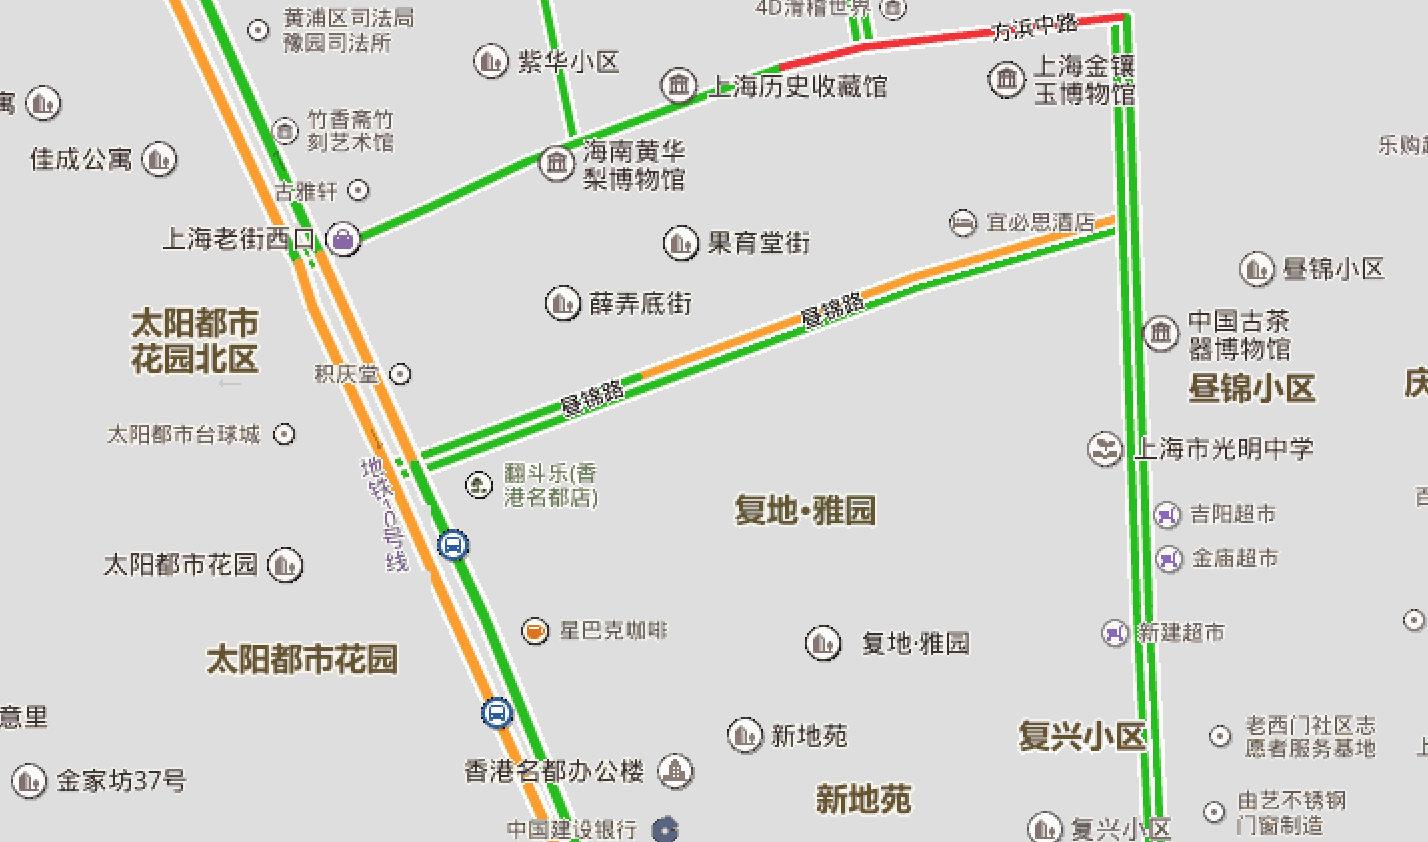
\includegraphics{figures/data/range.png}}
%	\caption{one range of our map}
%	\label{fig:range}
%\end{figure}
%
%The figure above consists of some small tiles as following.
%
%\begin{figure}[th]
%    \centering
%	\begin{subfigure}[t]{0.45\columnwidth}
%	\framebox{\resizebox{\columnwidth}{!}{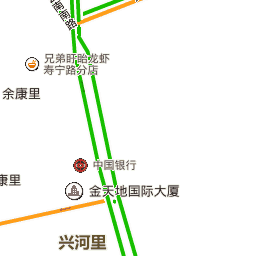
\includegraphics{figures/data/tile1.png}}}
%	\caption{}
%	\label{fig:tile1}
%	\end{subfigure}
%    \hfill
%	\begin{subfigure}[t]{0.45\columnwidth}
%	\framebox{\resizebox{\columnwidth}{!}{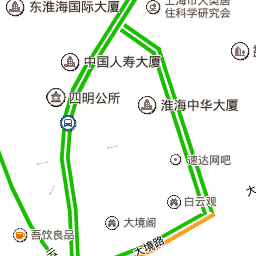
\includegraphics{figures/data/tile2.png}}}
%	\caption{}
%	\label{fig:tile2}
%	\end{subfigure}
%	\caption{Two tiles of our map}
%\end{figure}
With the (x, y) point coordinate in Baidu,  we can compute the exact
pixel in the traffic tile image downloaded from Baidu, using the following
equations. Here $point$ means either $x$ or $y$ in the point coordinate,
$pixel$ means either $x$ or $y$ in the image,
and $level$ is the zoom level of the tile image.

\begin{align}
tile & = \left \lfloor \frac{point \times 2^{level-18}}{256} \right \rfloor
\end{align}
\begin{align}
pixel &= \left \lfloor point \times 2^{level-18} - tile \times 256 + \frac{1}{2} \right \rfloor
\end{align}

%\subsubsection{Getting POIs}
%For POI, we can query them by a range from Baidu API and get all POIs with BD-09 coordinates and all information. Then we need to convert them by function f. So we can get all POIs with WGS-84 coordinates and all information at last.
%
%There is no need to talk about the details of the usage of {Baidu APIs}.

\subsubsection{Parsing Traffic Information}
%We first get the ways from our previously dumped OpenStreetMap data, 
%each way in the OSM data contains a series of nodes, 
%with longitude and latitude, and those nodes connected following certain 
%sequence number forms the roads and ways in the map. 
%We interpolate some points between consecutive nodes connected, 
%and get the coordinates of those in WGS-84 format. 
%A simple API is also provided by Baidu to convert WGS-84 
%(the international standard) coordinates to BD-09 (a proprietary 
%coordinated system used exclusively at Baidu Maps). 
%After converting coordinates from BD-09 to WSG-84, we employ the following
%formula to translate the longitude and lattitude into (x, y) tile coordinates
%used simple formula to calculate the exact pixel coordinates in the downloaded traffic tile images. 
%\KZ{I'm a little lost: it seems that all we need is to translate 
%road segment in OSM into the right (x, y) coordinates in baidu.
%To do that, we can just use the translation funcation directly? We
%talked about function f and g before.. This should be discussed
%more in-depths in the previous section.}
%
%Then we use naive algorithm that find the colored pixels within a distance 
%threshold in terms of pixels from the sample point calculated above. 
%If the point node belongs to a way that is one way tagged, 
%then the search ends after only one color line found within threshold. 
%Otherwise, two colored lines in most proximity to the point in direction 
%orthogonal to the direction of the way are searched and found 
%within threshold. Assigning those color line pixel matching results to 
%the sample line would finish the task of parsing the raster image format 
%of traffic data, and save them accordingly for later training use. 
%See Figure~\ref{fig:trafficmatch} for an example processing result 
%of the raster image traffic data. The background is the image 
%crawled and merged from several traffic tiles from Baidu Map. 
%Black dots are all the nodes from our OpenStreetMap database mapped 
%onto the location of Baidu Map. The red and blue dots are the 
%parsing result of the image searching for each node's nearby color 
%line pixel representing traffic information, and two of them 
%in a pair denoting they are two directions of a two-way road.
%Some black dots that are not on the road are some other type of way nodes, 
%like subway line which we are not taking care of.
%
%\begin{figure}[th]
%	\centering
%	\resizebox{\columnwidth}{!}{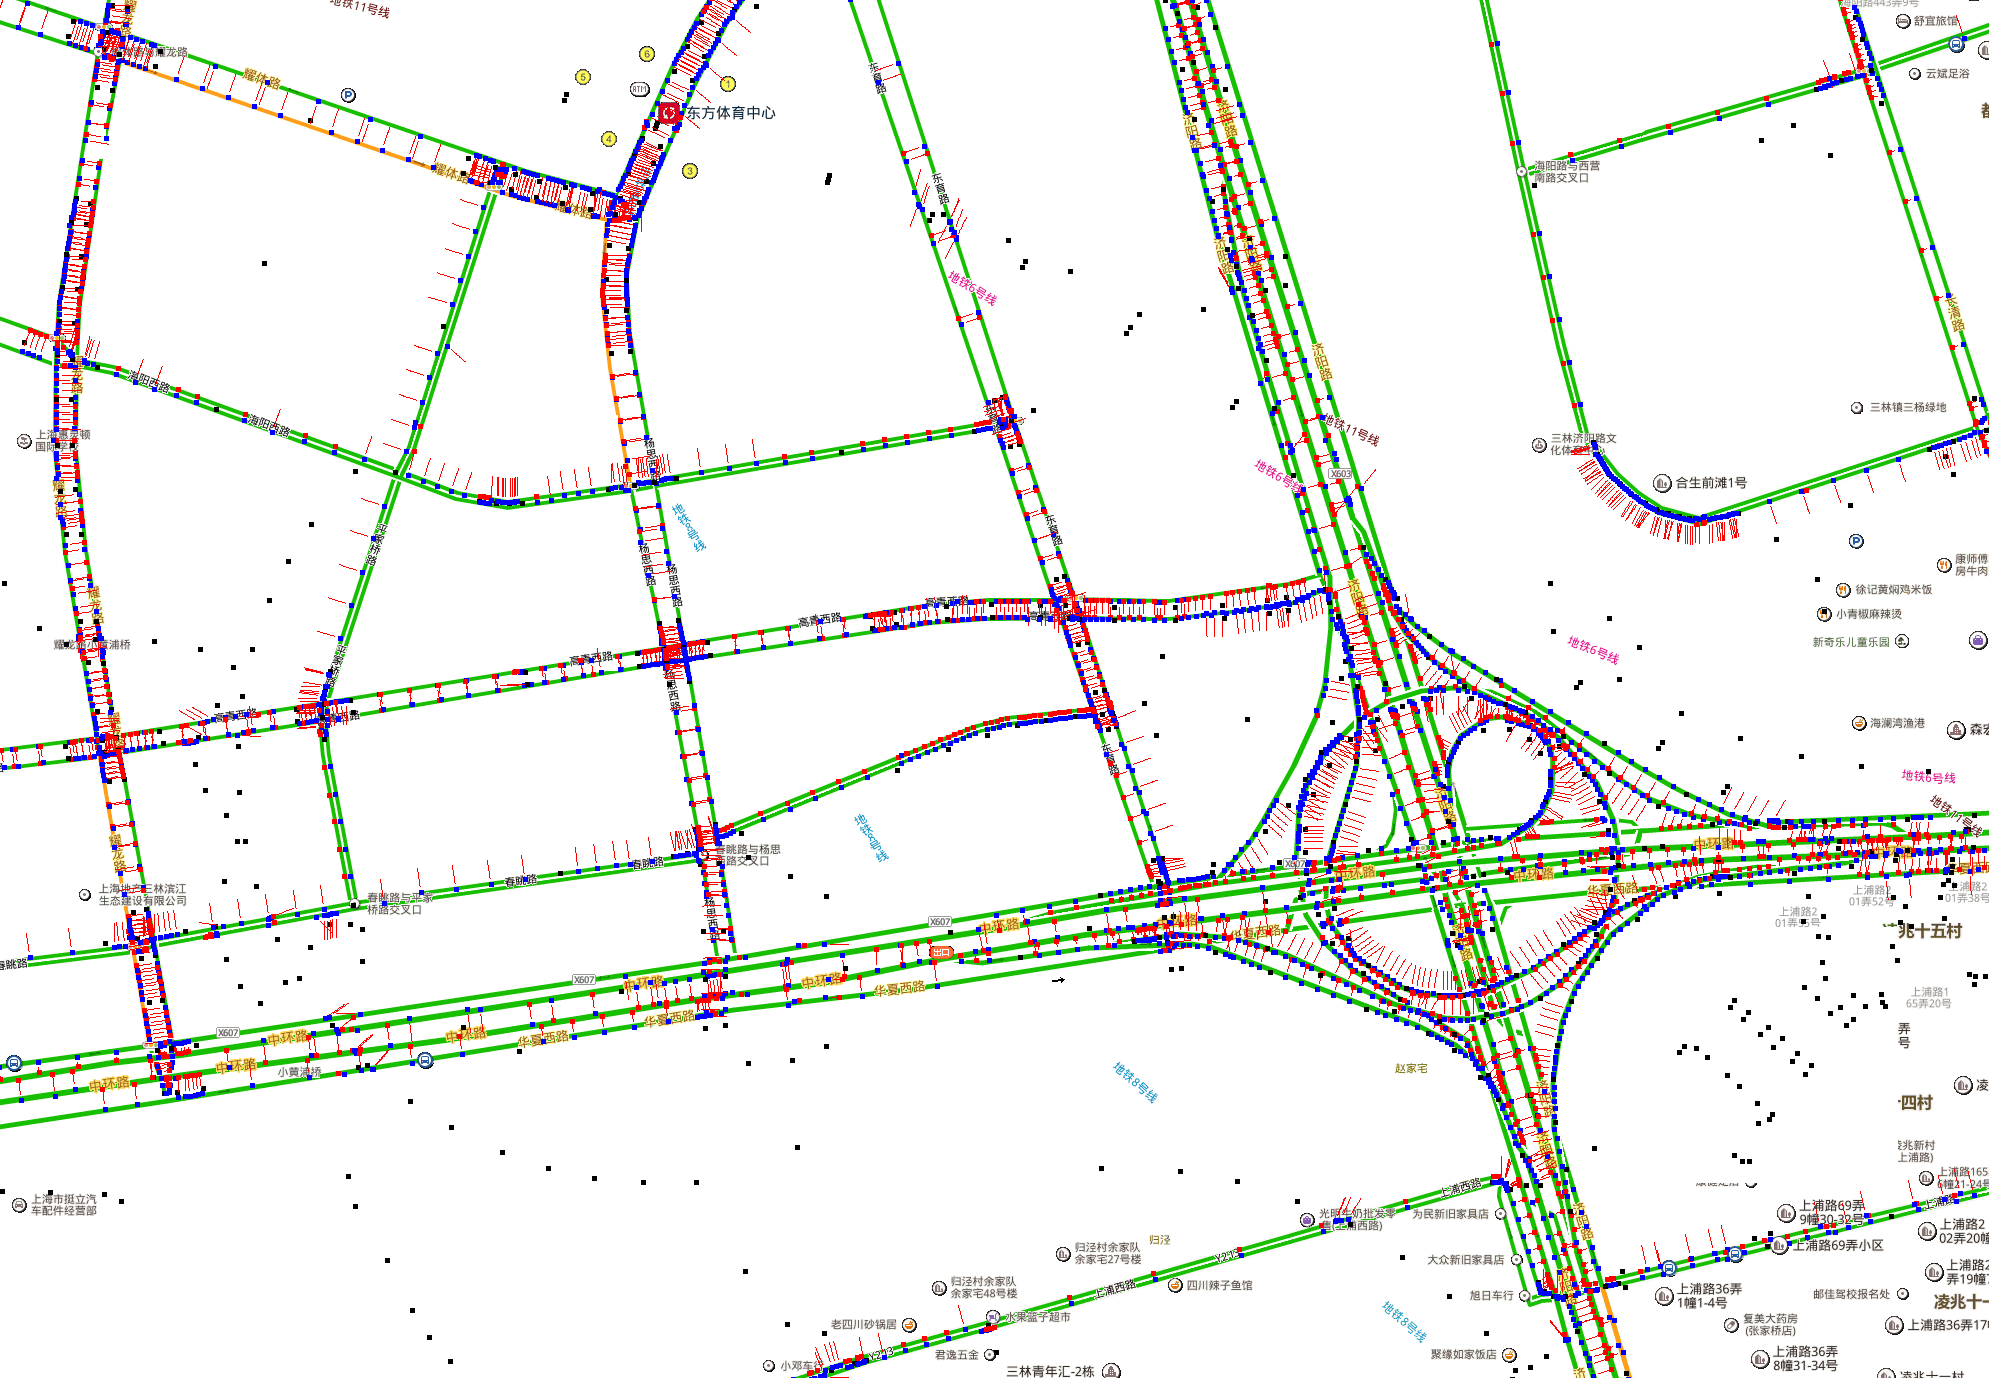
\includegraphics{figures/data/trafficmatch.png}}
%	\caption{An example traffic parsing process of part of the area. }
%	\label{fig:trafficmatch}
%\end{figure}
%
%\KZ{Replace \figref{fig:trafficmatch} with a zoomed in image.
%Add the figure in the defense slides to show how to get the colors from
%the target points.}

%We have all ways and nodes with WGS-84 coordinates and all information except traffic information of ways. So we need to get traffic information from Baidu for every ways. Obviously, we need both functions f and g which can locate any way's exactly position in Baidu Tiles, and parse the traffic information at last.

Despite all above efforts, the translation
from WGS-84 into Baidu's pixel coordinates is not perfect. 
Furthermore, the nodes along an OSM road is often mapped to the
center of the a two-way road (shown as the black dots in
\figref{fig:range}), where the traffic information (the
green, yellow or red lines) are painted on the sides of the road
(see \figref{fig:range}).
Therefore, in this section, we introduce our approach to fuzzy match
the nodes translated from OSM to traffic condition, that is the colored
pixels on the green, yellow or red lines.

\begin{figure}[th]
	\centering
	\resizebox{\columnwidth}{!}{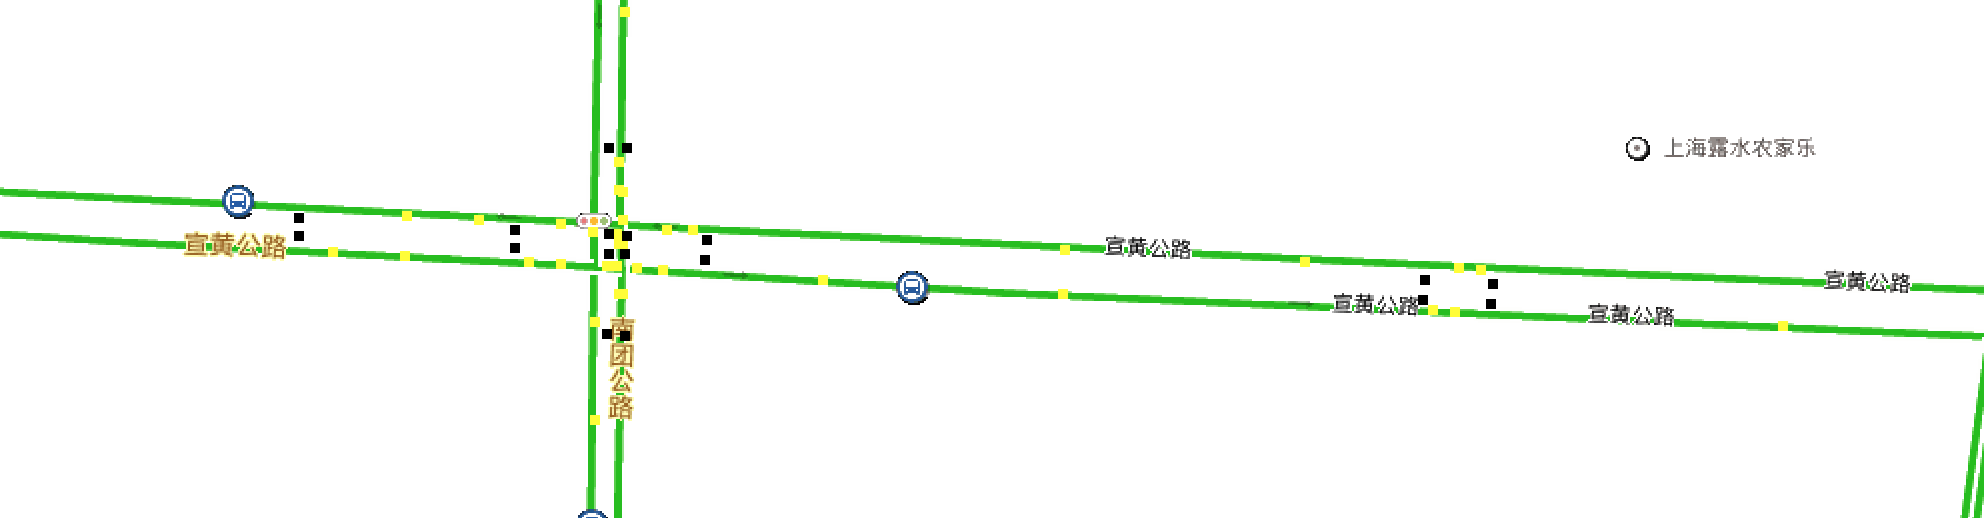
\includegraphics{figures/data/match_1.png}}
	\caption{Fuzzy matching example}
	\label{fig:range}
\end{figure}

We assume the road segment between two consecutive nodes $n_1$ and $n_2$ 
(shown as black dots in figure)
is a straightline and compute $n$ sample points on this line. 
The size of $n$ is proportional to the distance between  $n_1$ and
$n_2$. If this is a one-way road, we scan the pixels along the line
perpendicular to the road segment to look for nearst green, 
yellow, red or deep red color pixels
on the image within threshold distance. The four colors have standard
RGB values for Baidu map. If any of these colors is located, we have
found a {\em traffic sample}, and this is marked as a yellow dot
in \figref{fig:range}. By majority votes, the traffic samples for 
each road segment together decide the traffic condition of that segment.

The reason why we need to sample a number of points along every road 
segment is because sometimes roads are very close to each other 
and may introduce noises, such as the junction and ramps of 
two expressway depicted in \figref{fig:junction}. Also notice that
some roads from OSM on the lower right corner of the figure
do not have traffic information.

%The figure above is one example of Baidu Tile Ranges. Before parsing, we merge every range of tiles to one big image which can be parsed more simple and fast. But we have no enough memory to parse the whole image of HuangPu district of Shanghai. The partition of Baidu Tile Ranges should fit our ways' data and ensure both the integrity and speed. There has no need to talk about the details of this partition.
%
%Let's see this figure. Black points depends the origin nodes in Open Street Map's data, and yellow points depends the sample nodes of ways which can help us to parse the traffic information of ways. You can see that our black points are not exactly on the road lines of Baidu Map due to the coordinate transformation error. So there're many problems here.
%
%For any way, we sampled n nodes and did fuzzy parsing for its traffic information. At last, we compared all results and got a best traffic result for this way. This n is different which is depends on the length of this way. If n is too small, maybe all samples will be covered by some noises such as road name, parking mark and so on. And if n is too large, the speed of parsing will be too slow.
%
%In this figure, there has only oneway which samples of it are painted to yellow. You can see two horizontal ways in it. Then there has another figure following which has many ways which has two direction, we call it twoway:
%
%\begin{figure}[th]
%	\centering
%	\resizebox{1\columnwidth}{!}{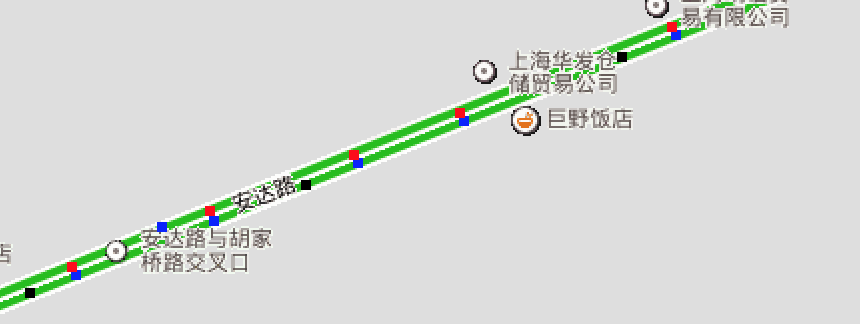
\includegraphics{figures/data/match_2.png}}
%	\caption{large amount of noises matching example}
%	\label{fig:range}
%\end{figure}
%
%This figure also has more noises on it. We computed the direction of sample list by Computation Geometry and believed in majority and good places to solve the noises. You can see a good recognition result in it.

\begin{figure}[th]
	\centering
	\resizebox{0.8\columnwidth}{!}{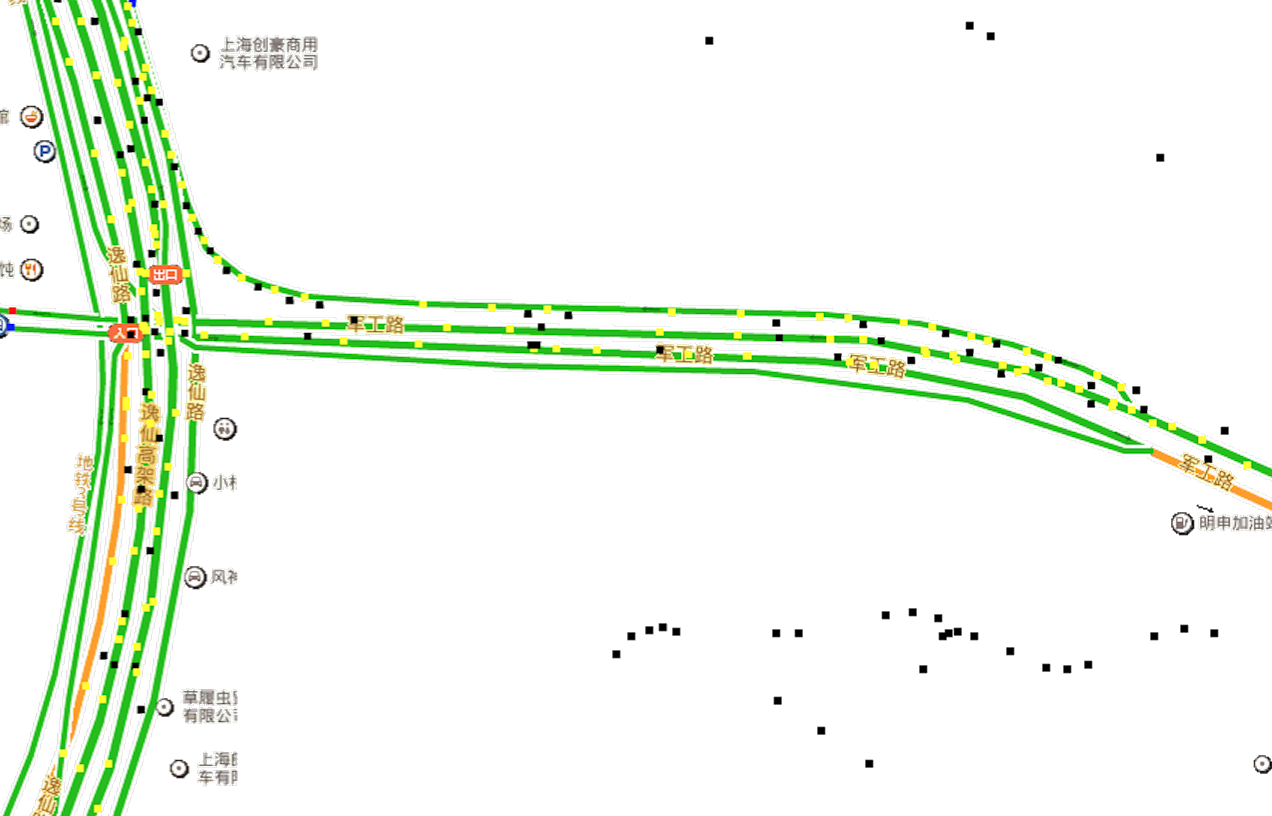
\includegraphics{figures/data/match_3.png}}
	\caption{Junction of expressways}
	\label{fig:junction}
\end{figure}

%There are many elevated roads which are very nearly, and some ways which hasn't traffic information in Baidu Map. We also has a good recognition for them.

For two-way roads, traffic conditions can be found on two directions
and this needs to be handled by looking for two parallel colored lines
nearby the sample points, indicated as red and blue dots in 
\figref{fig:elevated}.  Almost all traffic conditions are correctly
identified in this very complex scenario.

\begin{figure}[th]
	\centering
	\resizebox{1\columnwidth}{!}{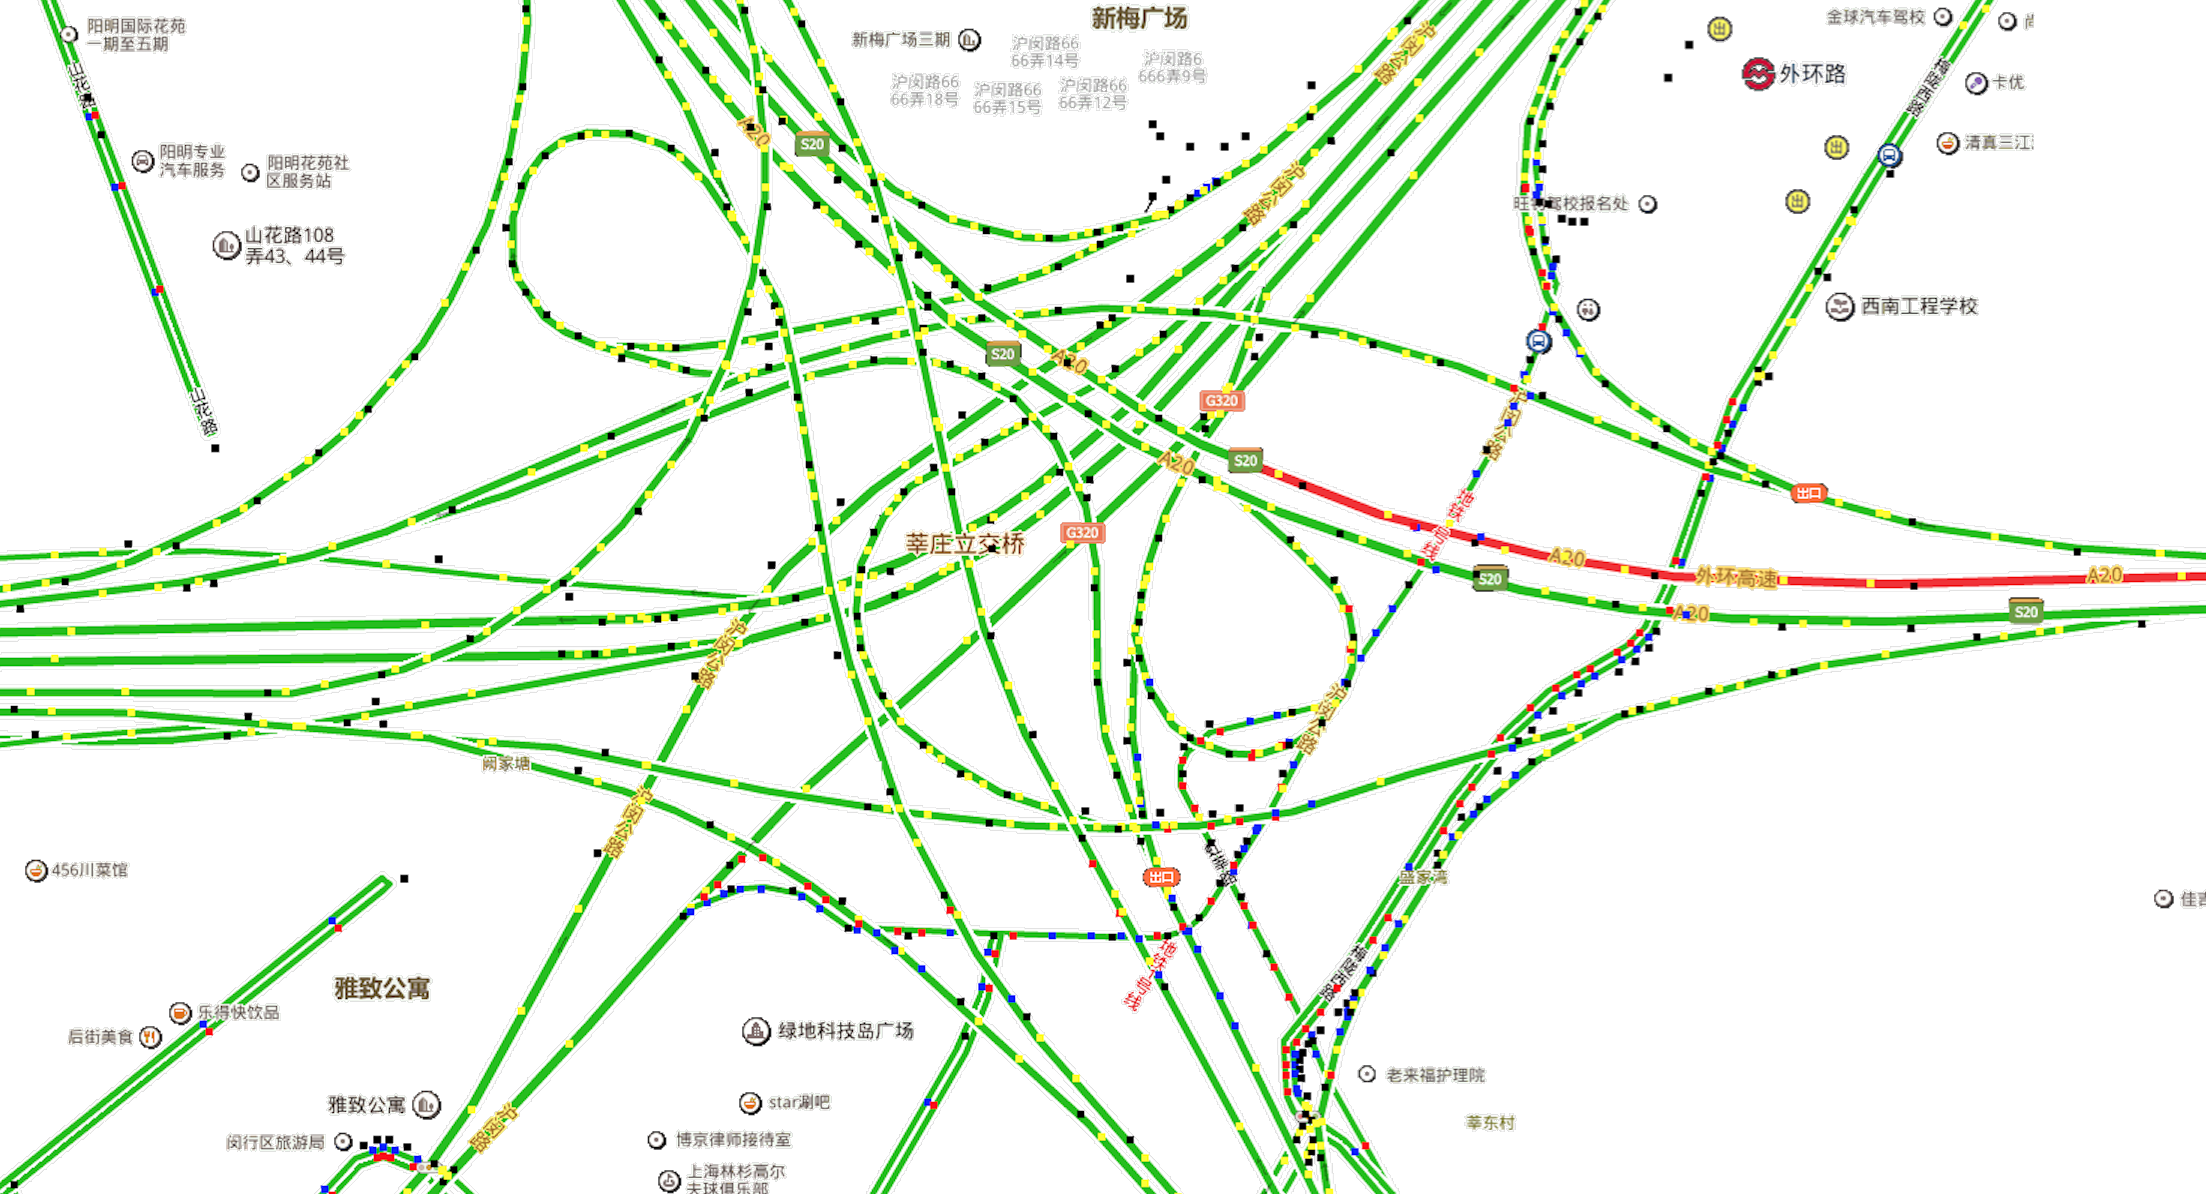
\includegraphics{figures/data/match_4.png}}
	\caption{Massive junction of elevated roads}
	\label{fig:elevated}
\end{figure}

%At last of this part, you can see crazy elevated roads here as one of the most complex conditions. As a conclusion, we solved the parsing perfectly and got all Traffic Information in Baidu Map.
